
\cleardoublepage


\chapter{Experimental Validation}


% introduction here
% ----------------------------------------------------------------------------


\section{Modeling}

\subsection{NEBP Decoupling}

% why model?
% can i use the full model?
% no, we need a decoupled model
% is it valid to decouple?
% yeah, as long as the coupled surfaces capture the outgoing flux, in our case that's justified because a vast majority comes down the beam
% what does the decoupled model include?
% well, i converted the tally into a source at the surface 
% the beam and space outside contain universes that different detectors can be included in
% the whole thing is wrapped and driven by python, too so that's great


\subsection{Gold Foil Tube}

% the foil tube was a type of spectrometer
% the gold foil tube design was based on the bonner sphere - thermal responsing detector with varying moderation
% produce independent responses
% it was also meant to help with beam alignment and to simplify the beam characterization process

%
%\begin{figure}[htb]
%\centering
%\includegraphics[height=4in]{tex/figures/.png}
%\caption[]{}
%\label{fig:}
%\end{figure}


% you can see the device in FIG
% there are three major components, the aluminum tube, the hdpe separators and the gold foils
% the gold foils are __ diameter and __ thickness
% the hdpe was cylinders of __ size
% each hdpe piece had a __ size hole drilled into it where the gold foil would be situated
% all of these would be encased in __ID __OD aluminum tubing
% aluminum is chosen because it's relative insensitivity towards neutrons
% the whole apparatus had __ hdpe pieces and foils, with the first foil being exposed and a gap of __ at the beginning

% this device was modeled in mcnp, where f4 flux tallies, folded with the au n,g response were used with a scx card to produce the rfs

\subsection{Bonner Sphere Spectrometer}

% a second, active detector was included in the experiment, too, the bss
% the bonner sphere spectrometer uses a series of plastic spheres surrounding a lithium iodide detector to produce independent responses

%
%\begin{figure}[htb]
%\centering
%\includegraphics[height=4in]{tex/figures/.png}
%\caption[]{}
%\label{fig:}
%\end{figure}



% you can see the device in FIG
% the full device was modeled using the 4x4 mm detection crystal coupled with pmt and hdpe sphere
% positioned a distance of __ from the bp aperture
% rfs were generated for sphere sizes of __ __ __ whatver
% the tally used f4 folded with the n,t reaction in the crystal with the scx card again



\subsection{Response Functions}

% describe any post processing used for these results to get the values in cm2

% add the plots and then discuss

% the gold foil tube response functions
\begin{figure}[htb]
\centering
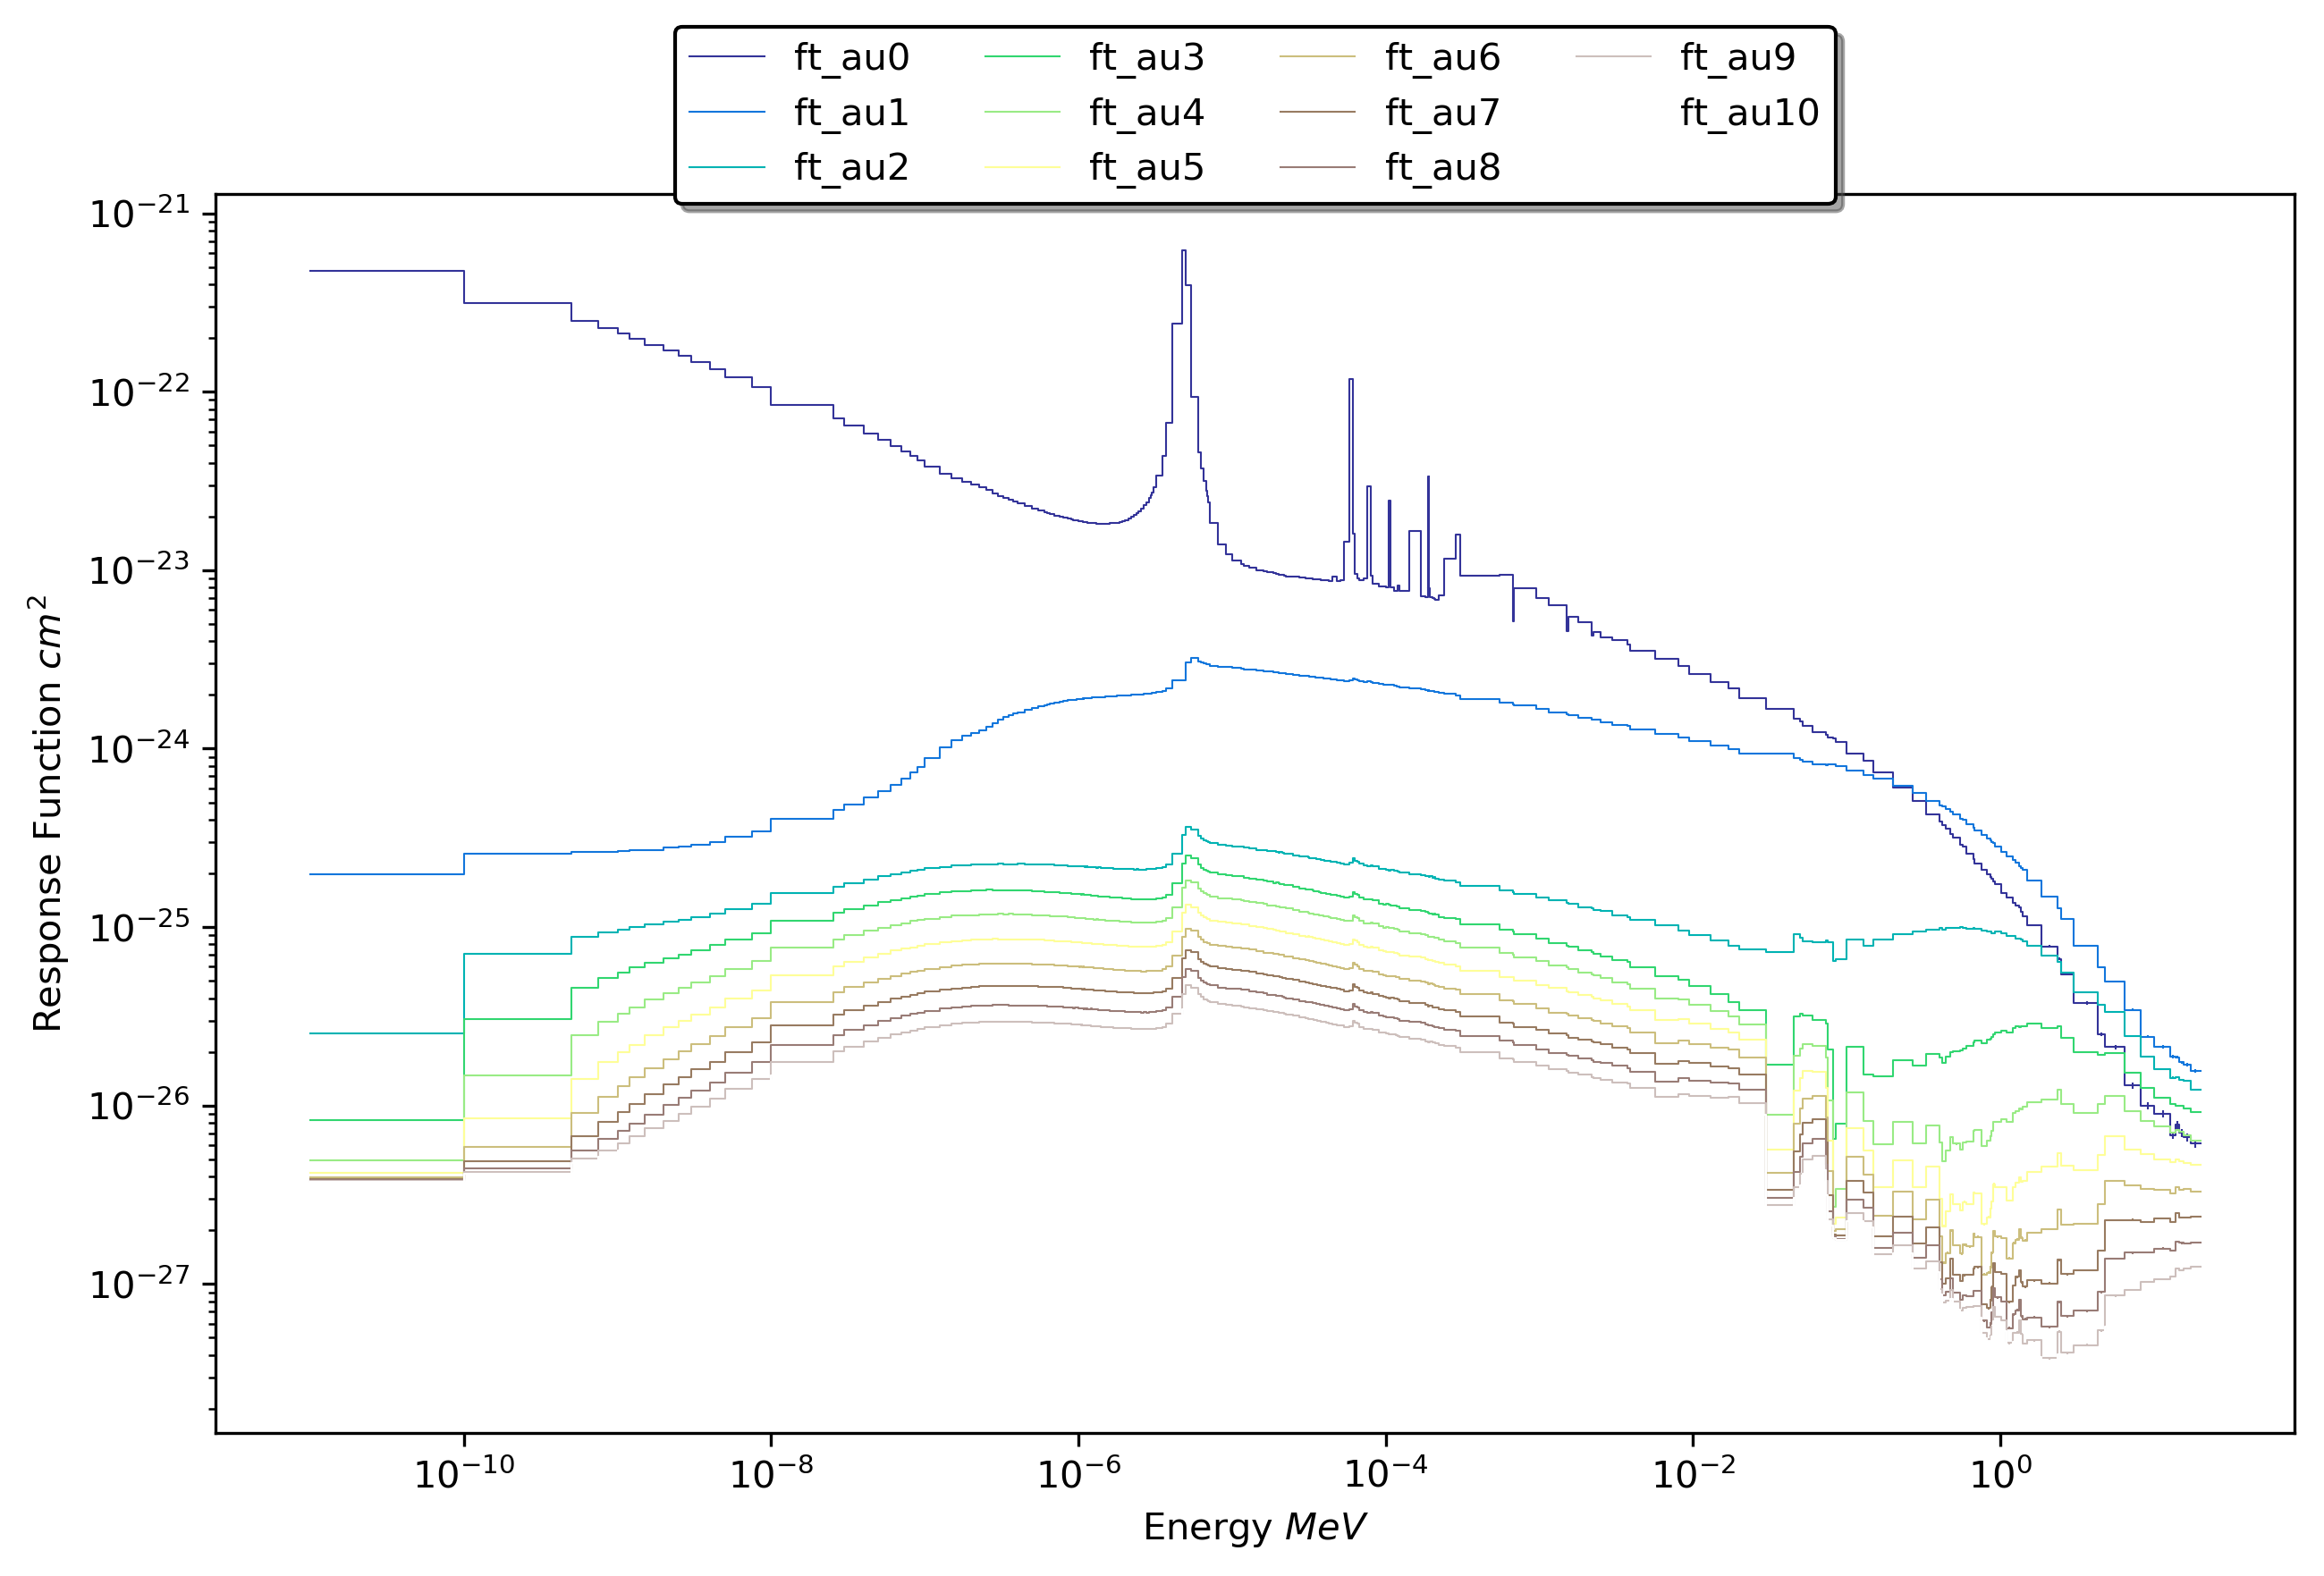
\includegraphics[height=4in]{tex/figures/ft_au.png}
\caption[Gold Foil Tube Response Functions]{The response functions for the gold foil tube.}
\label{fig:ft_au_rfs}
\end{figure}

% discuss the ft_au response functions

% the bonner sphere response functions
\begin{figure}[htb]
\centering
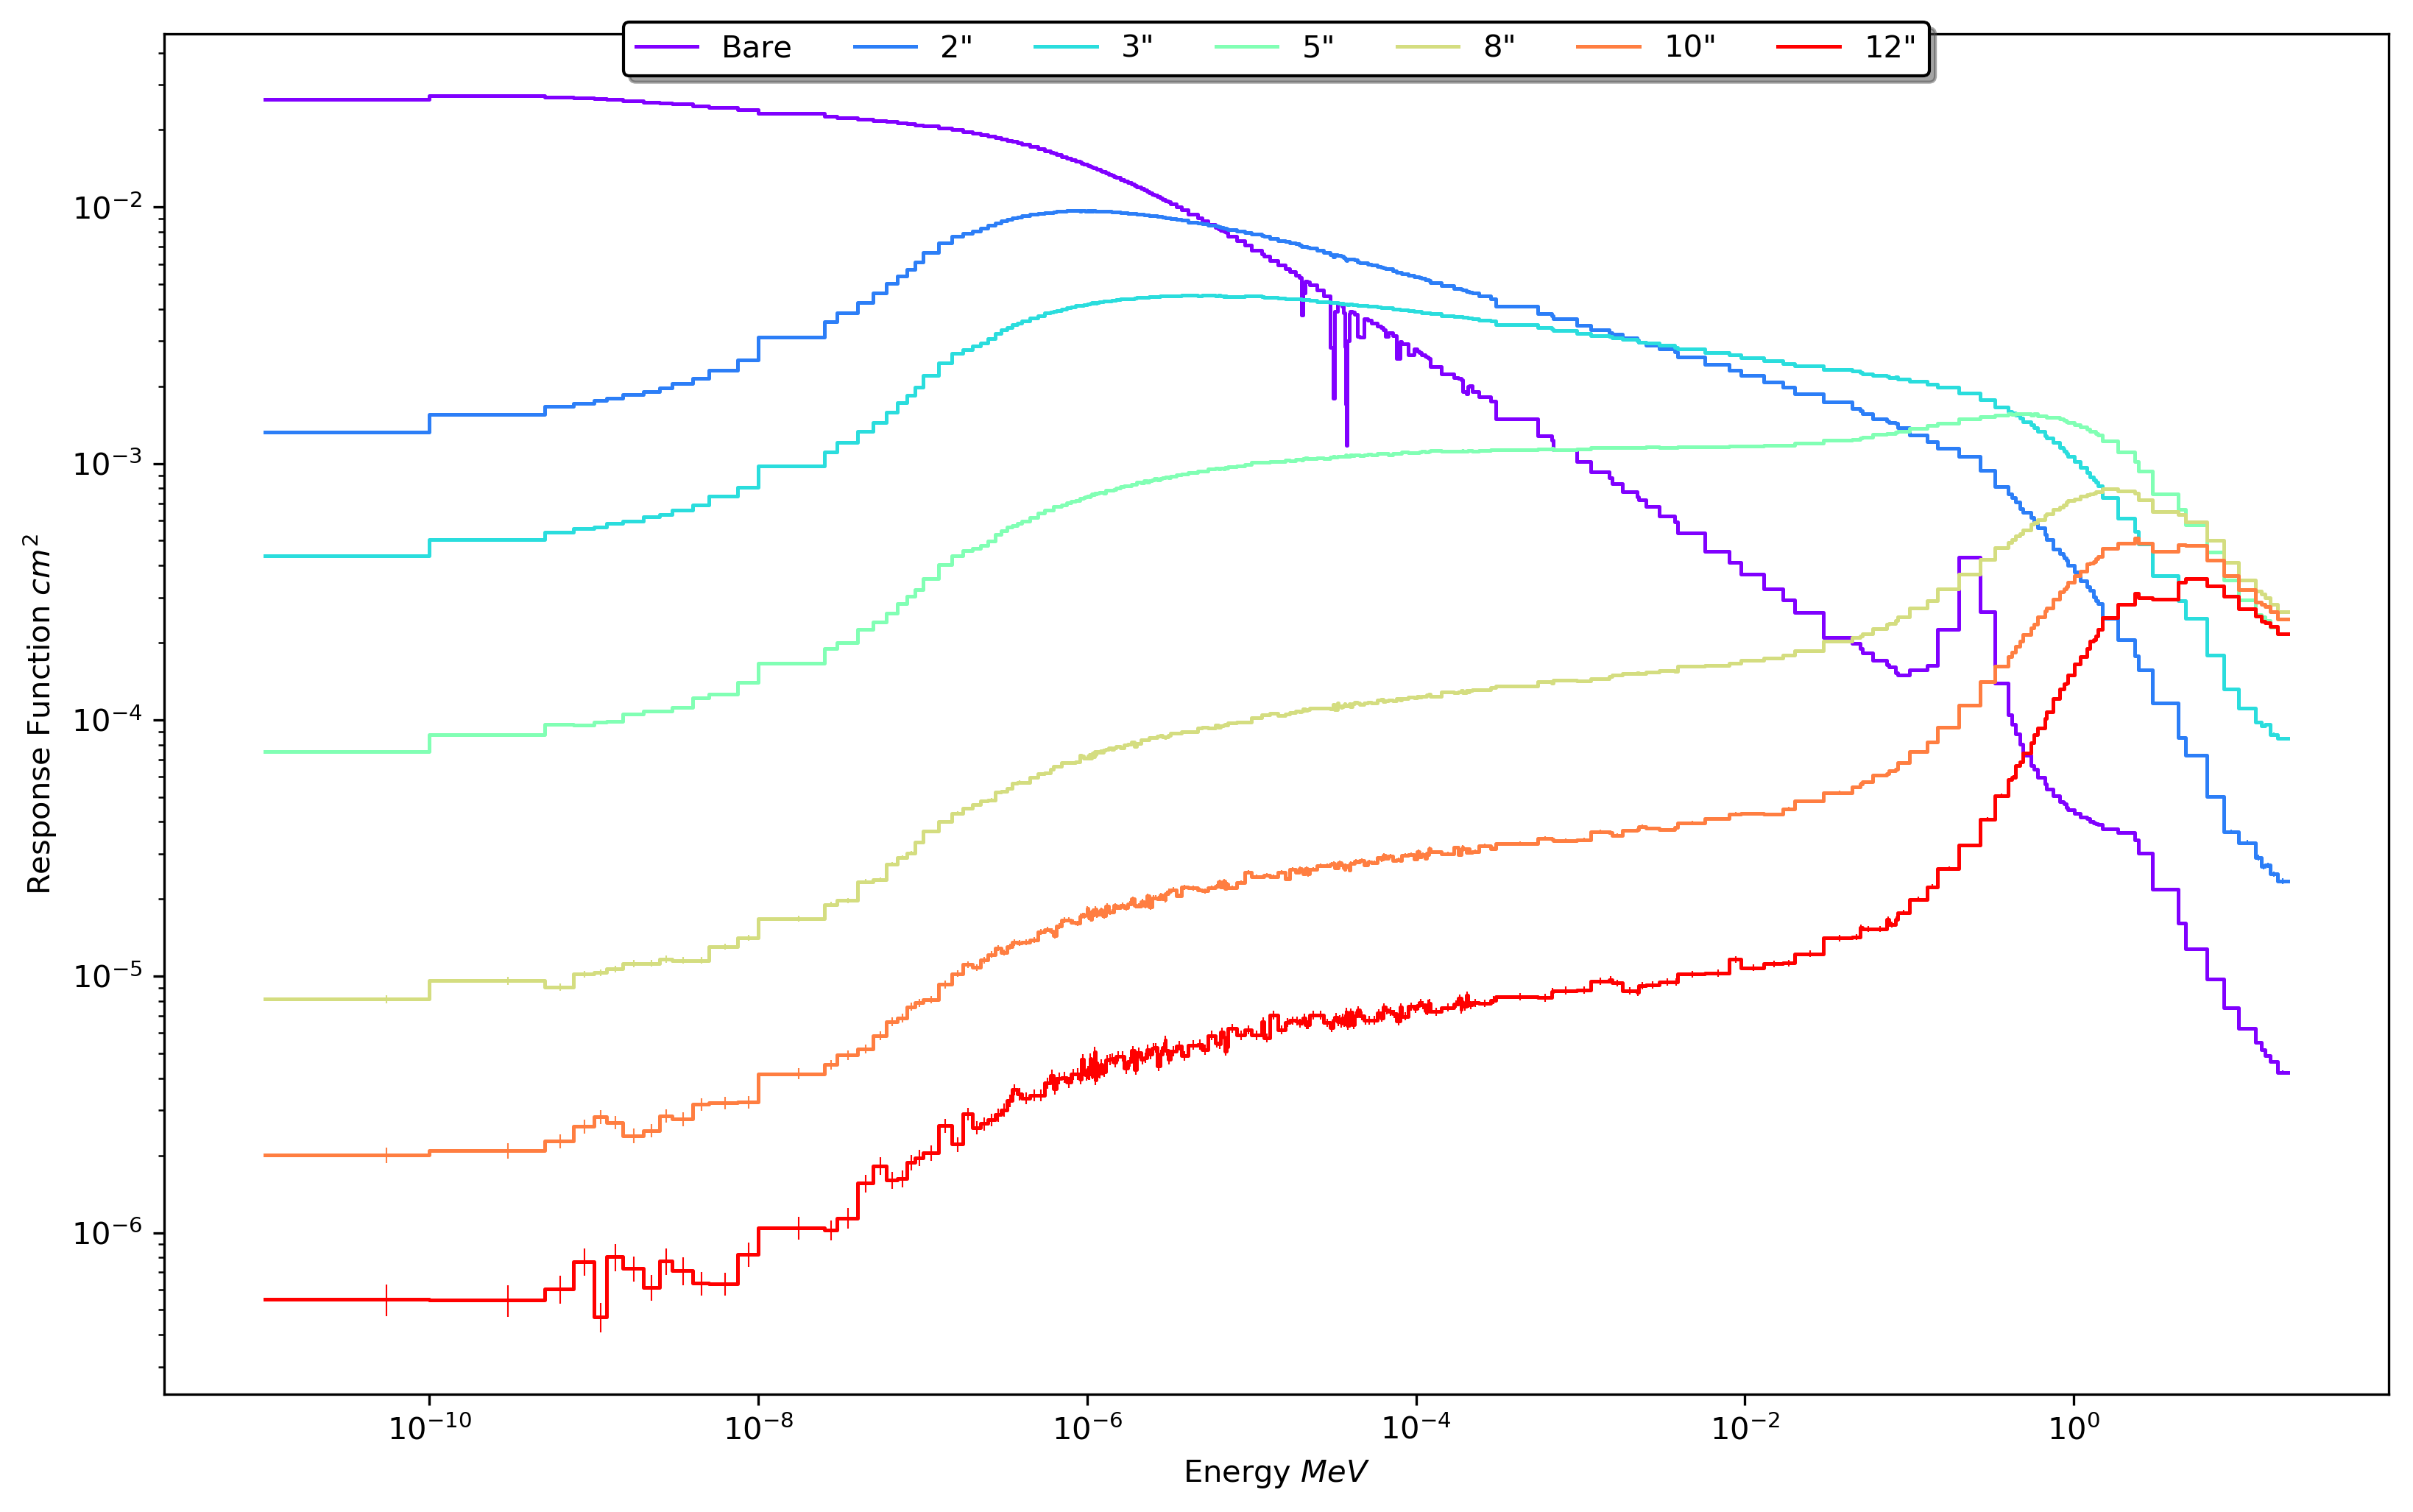
\includegraphics[height=4in]{tex/figures/bs.png}
\caption[Bonner Sphere Spectrometer Response Functions]{The response functions for the Bonner Sphere Spectrometer.}
\label{fig:bs_rfs}
\end{figure}

% discuss the bss response functions

% ----------------------------------------------------------------------------
% other stuff here
